\section{Realizing the Method with Subgraph Execution}
\label{sec:execution}
The dependency construction specifies legal work and communication but leaves
their physical implementation open. This distinction lets the same method
use a register codelet, a cooperating warp, or a block-local core without
making any one of them part of the mathematical definition. A realization
binds each dependency-closed subgraph to a core, storage scope,
and schedule. The core implements its stage bits, arithmetic, and coefficient
rules while declaring value ownership and local synchronization. Register
codelets, warp cooperation, block-local kernels, and imported components can
satisfy this contract with different resource costs.

The interface must describe more than the number of input values. A core
also declares their logical roles, which threads own them, and the
synchronization required before its outputs are visible. These requirements
connect the core to the surrounding layout and schedule. Replacing a core
can change the best organization even when the two compute the same function,
because their registers, shared storage, and exchange patterns differ.

\subsection{Successor-aligned writeback}
The first physical problem appears when a locally efficient producer leaves
its outputs in an inconvenient representation for its consumer. An explicit
permutation is always a possible implementation, but adds a pass over the
boundary data. Instead, the producer can incorporate the required placement
into its writeback when its ownership and store pattern permit it.
A producer's output representation must agree with the successor's input
representation for each logical value $i$,
\begin{equation}
\lambda_{\mathrm{out}}(i)=\lambda_{\mathrm{in}}(i).
\label{eq:handoff}
\end{equation}
Together with compatible ownership and publication, this is the
\textbf{successor-aligned writeback} rule. It can remove a separate
permutation by placing values for their next use.

One construction moves the successor's variable stage bits into low-order
address positions, placing its component in a contiguous range. In the
Hadamard example, a producer can write logical index $4r+c$ at address
$4c+r$, so the next band reads a column contiguously. Identity placement and
explicit permutation remain alternatives. Consumer locality alone does not
guarantee efficient stores, so the candidate cost includes both transactions
and any staging.

Shared storage adds a bank constraint. For an illustrative square tile with
power-of-two side $P$, $P$ banks, and one word per value, consider
\begin{equation}
\lambda(r,c)=P\,r+(c\mathbin{\oplus}r).
\label{eq:swizzle}
\end{equation}
XOR by a fixed row is a permutation. Under the single-word access pattern in
Figure~\ref{fig:banklayout}, both a row and a column reach distinct banks.
Vector values and partial warps require their actual transaction analysis.
Global layouts obey the same value-identity rule but are evaluated for
alignment, transaction width, and coalescing.

\begin{figure}[t]
\centering
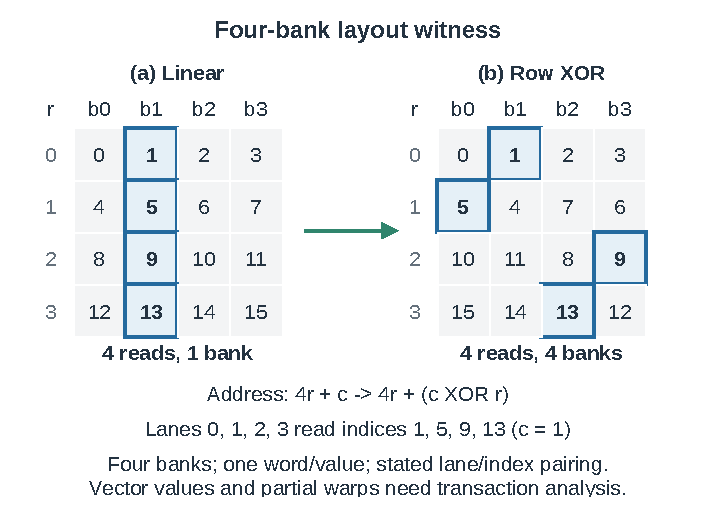
\includegraphics[width=\columnwidth]{figures/drawio/exports/bank_layout.pdf}
\caption{A four-bank layout witness. A row-dependent XOR offset distributes
a logical column across banks for the stated single-word access pattern.}
\label{fig:banklayout}
\end{figure}

\subsection{Residency, publication, and finite buffers}
Correct placement alone does not make a value ready. The row/column example
requires contributions from several producers, and reusing a buffer too early
would overwrite data still needed by a consumer. Execution therefore tracks
availability and lifetime at the same dependency granularity as the handoff.
A resident group tracks its live values and unfinished consumers. A
materialized boundary publishes a dependency unit, and the successor starts
only when its predecessor set is ready. A buffer slot is acquired before
writing, published after production, and released after the last required read.
The slot count trades lookahead against live state and synchronization cost.
Tail tiles retain their actual shape and release event.

Figure~\ref{fig:pipeline} illustrates the distinction with independent
Hadamard transforms. Completing one row leaves every column waiting for
three other rows. After the full row band publishes, its column consumers
can overlap the row work of another transform if resources permit. The
buffer holding the first transform becomes reusable only after its final
consumer read, not simply when its producer has finished.

These rules support bulk execution and pipelines across storage scopes.
Independent transforms may interleave, while a row-to-column boundary within
one transform retains its fan-in constraint. Larger batch supplies scheduling
opportunities, but legal overlap still depends on readiness, resource
availability, and buffer lifetimes.

\subsection{Composing physical services}
Once placement and lifetime are fixed, the remaining performance question is
how the local work composes. Summing isolated core times misses startup and
boundary work, while assuming ideal overlap ignores readiness and contention.
We use the actual physical groups and release rules to distinguish these costs.
For a selected physical group, a \textbf{service model} separates startup,
repeated work, and the tail,
\begin{equation}
T_{\mathrm{group}}=T_{\mathrm{start}}+R\,T_{\mathrm{step}}+T_{\mathrm{tail}}.
\label{eq:serial}
\end{equation}
The terms depend on the core, tile shape, layout, launch geometry, and storage
scope. A complete-kernel measurement already includes its launch and tail.
Bulk execution sums group services plus boundary costs not already included.

For $K$ tiles in a repeatable pipeline, the corresponding view is
\begin{equation}
T_{\mathrm{pipe}}\mathrel{\approx}T_{\mathrm{fill}}+(K-1)\,\mathrm{interval}
                  +T_{\mathrm{drain}}.
\label{eq:pipeline}
\end{equation}
Ready dependencies, finite-buffer reuse, and shared execution or memory
resources limit the interval. Overlapped groups need not retain their isolated
service rates. More independent work amortizes fill and drain and can cover
transfer latency, but cannot exceed a saturated resource's throughput.
The model ranks realizations under these assumptions rather than proving
optimality.

\begin{figure}[t]
\centering
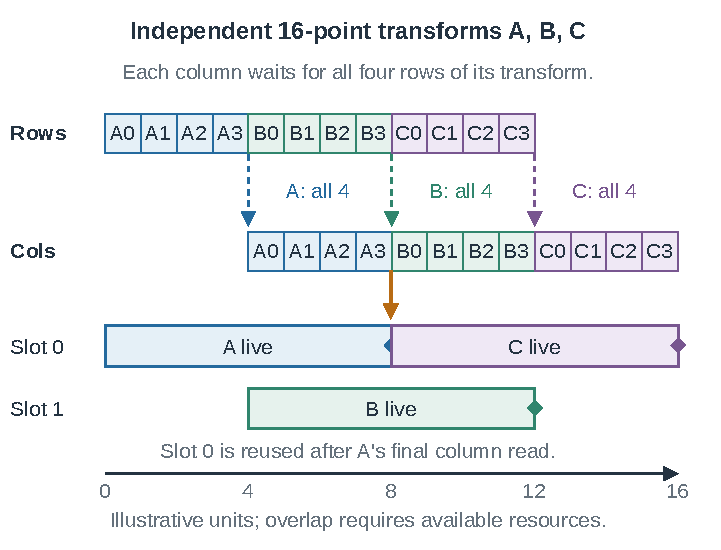
\includegraphics[width=\columnwidth]{figures/drawio/exports/pipeline.pdf}
\caption{Readiness and lifetime for independent 16-point Hadamard transforms
A, B, and C. Each column requires all four rows of its transform. Slot 0
becomes reusable by C only after A's final column read. Equal operation
durations are illustrative, not measured. Lanes denote logical work, and
cross-transform overlap requires available resources.}
\label{fig:pipeline}
\end{figure}
